\documentclass[12pt,a4paper]{article}
\usepackage[utf8]{inputenc}
\usepackage{amsmath}
\usepackage{amsfonts}
\usepackage{amssymb}
\usepackage{graphicx}
\usepackage{booktabs}
\usepackage{natbib}
\usepackage{dcolumn}
\usepackage{setspace}
\usepackage{array}
\usepackage{pdflscape} %allows for rotating pages with wide tables
\newcolumntype{P}[1]{>{\raggedright\arraybackslash}p{#1}}
%\usepackage{tabulary}
\usepackage[T1]{fontenc}
\usepackage{lmodern}
\usepackage{multirow}
\usepackage{multicol}

%\usepackage{mathptmx} %times font
%\usepackage{tgtermes} %times font
\usepackage[protrusion=true,expansion=true]{microtype}
\usepackage[top=1in, bottom=1in, left=1in, right=1in]{geometry}
\usepackage{hyperref}
\usepackage{color,soul} %highlighting
\usepackage{caption}
\captionsetup[figure]{labelfont=bf}
\captionsetup[table]{labelfont=bf}

%\usepackage{endnotes}
%\usepackage[heads,nolists,tablesfirst]{endfloat} %places tables and figures at the end
%



\usepackage{epstopdf}

\title{\textbf{Housing Bubbles and \\Support for Governing Parties}}


\author{
Frederik Hjorth \and Martin V. Larsen}

%, \textt{fh@ifs.ku.dk}, (+45) 26 27 24 41 }  } 


\begin{document}

\maketitle

\begin{center}
\textsc{draft - please do not quote, cite, or circulate}
\end{center}

\begin{abstract}
\noindent When the real estate bubble burst in 2007 it had profound consequences for the state of the world economy. However, we know little about whether or how this housing bubble affected voting behavior. Studying the electoral consequences is important, because it helps us understand how voters react to economic shocks which affect their immediate environment and, in turn, the incentives reelection-minded politicians face when trying to deal with economic bubbles. In this paper, we zoom in on one country, Denmark, a country which had exceptionally volatile house prices, and examine how this rapid expansion and contraction of real estate prices shaped support for governing parties across four parliamentary elections. To do this, we link detailed data on local house prices to election returns at the precinct level. Across a wide range of demanding specifications, we find that the when house prices change so does the governing parties vote share. Further, this relationship seems to be stronger in areas where house prices are very volatile, and when the change in house prices are negative.
 
\end{abstract}

%\begin{keyword}
%\doublespacing
%%x \sep y
%\end{keyword}

%\end{frontmatter}

\newpage

%\onehalfspacing
\doublespacing

\section{Introduction}
In this article we examine how local house prices shaped the electoral success of governing parties in Danish parliamentary elections from 2005 till 2015. A period in which the real-estate market in Denmark experienced a dramatic boom and bust \citep{dam2011housing}. Specifically, we want to examine whether voters held governing politicians electorally accountable, in the sense of electorally punishing and rewarding them, for changes in house-prices in their community. That is, whether a decline in house prices in a community means that voters in this community are less likely to support governing parties. 

Compared to other features of the economy, the quality and status of one's home has recieved scant attention in extant literature on economic voting. A small literature exists on patrimonial economic voting \citep{nadeau2010patrimonial,stubager2013reaching}, that is the extent to which owning assets, like real estate, makes it more likely that you will vote for right-wing parties \citep[see][for a similar argument]{ansell2014political}. However, very few studies and have focused on whether house prices, similarly to other economic indicators like unemployment and GDP per capita, influence electoral support governing parties. Further, in the few studies which do include house prices, the effects of these house prices rarely examined in details.  \citep[e.g.]{hopkins2015economic}. 


Understanding how the housing bubble affected support for governing parties is important for, at least, two reasons. First of all, just like we learn something political business cycles from studying voter myopia \citep{healy2014substituting,tufte1980political}, or learn something about the prevalence of disaster relief vis a vis disaster preperation spending by looking at how voters reward spending on one or the other \citep{healy2009myopic,ashworth2012electoral}, studying how voters react to housing bubbles tells us something about the political antcedents of these bubbles. Specifically, it highlights the incentives reelection-minded politicians face when developing policies which influence the formation of economic bubbles

Second of all, studying house prices allows us to understand how local economic conditions shape electoral support for governing politicians. Something which is interesting in light of the fact that most studies of the electoral effects of the economy has focused on the national economy or, to a lesser extent, personal economic conditions \citep[290]{healy2013retrospective}. To the extent that we find that voters do hold politicians accountable for economic conditions in the local context, this means that politicians cannot simply be attentive to economic conditions as a whole, but has to worry about the geographic distribution of these conditions \citep[cf.][11]{ferejohn1986incumbent}. 

A number of existing studies have examined the political effects played by local economic conditions. A set of studies have looked at whether local economic conditions affect voters perception of the national economy; they generally find mixed or small effects (\citealt{books1999contextual,reeves2012ecologies,anderson2011local,ansolabehere2014mecro}; although \citealt{dinesen2015reconsidering} find substantial effects). Another set of studies have looked at consequences for support for governing parties, finding mixed or statistically insignificant effects of local economic conditions \citep{hansford2015reevaluating,eisenberg2004economic,kim2003spatial}. As such, the existing literature has not been able to show strong effects of local economic conditions. This might mean that they are not at all important for voters. However, it might also mean that previous literature has simply been unable to identify these effects. There are some issues with the data and methods used in previous research, which suggest that the latter might be true.

First, previous literature have  generally relied on rather large geographical units (e.g. US counties) when estimating the effects of local economic conditions. This is potentially problematic, as the local context voters react to, might not map on to these large geographical areas. Second, the studies do not generally take structural differences between local contexts into account when relating economic conditions to  attitudes or voting behavior. This is potentially problematic, since it seems likely that voters will, at least take some structural factors into account. In the present case, voters are probably not likely to infer much about the government based on the fact, that there are differences in house prices between cities and rural area. They are more likely to infer based on the fact that their house prices are declining, or that they are not rising less than they usually do. Related to this, one risks conflating re-distributive concerns, i.e. voters in comparatively less well of areas having different demands from government than those in well of areas, with inferential concern, what does my local context tell me about the national economy or about the quality of the government.  Third, the measures of local economic conditions are often based on samples which, while large enough to estimate precise national economic conditions, are not sufficiently precise on geographical levels. Taken together, these factors make it likely that previous studies do not estimate an reasonably efficient estimate of the effect of local economic conditions. 

In the present study we address all of these shortcomings by (1) using data on a small geographical level of aggregation (precints), (2) using panel data which removes any context-specific and time-invariant confounders and (3) using detailed register data from the Danish Mortgage federation on the actual price of all houses sold in the period under investigation. 

Analyzing these data, we find that changes in house prices do lead to changes in support for governing parties. A relationship which is quite robust. Further, we find that voters react more strongly to negative changes in house prices than positive changes, and that the effect is larger in areas where house prices have been especially volatile in the past. 

This heterogeneity in the effect of house prices makes sense given previous literature on the economic vote. As such, studies have long found that economic conditions matter more for election results when they are deteriorating \citep[e.g.]{bloom1975voter,headrick1991attention,nannestad1997grievance}. Further, to the extent that less volatility means that the policy-elasticity for house prices in this area is low, it makes sense that these prices also have a smaller effect. That is, if the effects of policy does not easily translate into outcomes (i.e. prices) in these areas, previous research suggests that outcomes should have a smaller impact on incumbent voting \citep{duch2008economic}.

What implications do these findings have? Most importantly, politicians should care about house prices and the policies that influence them.  Further, the asymmetry in responses to negative and positive changes means that politicians seemingly have little incentive to create housing bubbles. These results suggest that the rewards for rising house-prices are minimal, yet the punishment if the bubble bursts are quite large. Relatedly, they are more likely to be punished for the quality of house prices in more volatile areas, and since bubbles create volatility. More generally, these findings suggests that it might be interesting to look more at house prices as a driver of political behavior.

Before moving on it is important to note an important limitation of the present study. What we find is an aggregate level correlation. As such, we run into an ecological inference problem. Specifically, it is important to determine whether voters punish and reward the government for the quality of local house prices  because (1) their own house loses some of its value (egotropic), (2) they fear for the future of their community (geotropic) or (3) they infer something about the state of the national economy from their local area (sociotropic). However, given the state of the extant literature on house prices and the effect of the local economy, simply establishing an effect and describing how this effect varies seem to be a substantial step forward. 

\section{Empirical Setting}

In this study we focus on how the housing bubble affected support for governing parties in Denmark. Denmark is privileged as a case for two reasons.

The first is that Denmark had a very large housing bubble. As \cite[][49]{dam2011housing} explain concerning the housing bubble of the late 2000's ``developments in the Danish housing market in those years were unusually hectic, both in a historical and an international perspective.'' This is also evident from the figure below, adapted from their paper. The second reason we focus on Denmark, is that it is possible to obtain MORE



\begin{figure}
	\includegraphics[width=0.8\textwidth]{../figures/intcomparison}
	\centering
	\caption{Taken from \citep[50]{dam2011housing}}
\end{figure}



Turning to the political context, the government in the entire period we investigate (2005-2015) consisted of two different parties. From 2001 to 2011 the Liberal party was in government along with the Conservative party, and from 2011 till 2015 the Social Democratic party and the Liberal party was in power.\footnote{An additional party, the Socialist party, was in government from 2011 to 2013, however, since this party left government before the election, it is excluded when looking at electoral support for the governing party. To get data on electoral support at the previous election, we also use some data from the 2001 election in which the Social Democratic party and the Liberal party was in power.} 


\section{Data}
The key dependent variable in our study is percent of votes cast for parties in government in each voting precinct.\footnote{Results similar for only using prime minister party} This is measured for all precincts in five elections; 2001, 2005, 2007, 2011 and 2015. A number of precincts are redistricted between each election. This is problematic as we want to use  the precincts as part of a panel data set. There are two ways to deal with this. We can drop precincts, as their geographical boundaries get altered. This would mean dropping roughly 15 pct. of the data on the dependent variable. The other option is to fix the precincts geographical boundaries at one reference election (i.e. 2015), and then recalculate vote returns in any changed precincts, so they match up with the precincts in the reference election.  As many of the changes in geographical boundaries are minor, we opt to do the latter (for details of how returns from the redistricted precincts are calculated see xx). \footnote{We will eventually show results for the other option in an appendix. Turns out its not super important for the results}. 

The key independent variable is house prices. Remember to describe volatility measure. MORE

In addition to this we measure a number of structural factors. These are population based measures of economic characteristics of the precincts, which are originally from Statistics Denmark. These are only available at one point in time (2011), and as such cannot be modeled dynamically. the variables are income, average household income in the precinct in DKK,  employment, the percentage of people in the precinct who are on the job market, benefits, the percentage of people in the precinct who are on unemployment benefits (``kontanthjælp'' and ``dagpenge''), and wealth, average household wealth in the precinct in DKK.  


\section{Results}
In order to examine the relationship between electoral support for governing parties and one-year changes in local house prices, we estimate a set of linear regressions in table \ref{tab1}. In model 1 we simply look at the bivariate correlation. In model 2 we include precinct fixed effects to take precinct-specific and time invariant confounders into account. In model 3 we include year fixed effects to control for time trends. Finally, in model 4 we include year by structural factors interactions (i.e. income, wealth, employment, benefits by year dummies). This final model allow these important structural characteristics, which do not vary from election to election, to have different slopes across different elections. The standard errors are robust and clustered at the precinct level.

As can be seen from table \ref{tab1}, there is a statistically significant and positive effect estimate of one-year changes in house prices, indicating that a larger fraction of the electorate casts their vote for governing parties in precincts where house prices increase. In the most demanding specification, model 4, the effect is roughly 0.05. this signifies that if house prices increase one percentage points, governing politicians get 0.05 percentage point fewer votes. A small but meaningful average effect.



\begin{table}[htbp]\centering
\def\sym#1{\ifmmode^{#1}\else\(^{#1}\)\fi}
\caption{Estimated effects of house prices on electoral support for governing parties.} \label{tab1}
\begin{tabular}{l*{4}{c}}
\hline\hline
                    &\multicolumn{1}{c}{(1)}        &\multicolumn{1}{c}{(2)}        &\multicolumn{1}{c}{(3)}        &\multicolumn{1}{c}{(4)}        \\
\hline
$\Delta$ house price&        0.10\sym{**}&        0.12\sym{**}&        0.05\sym{**}&        0.05\sym{**}\\
                    &      (0.01)        &      (0.01)        &      (0.01)        &      (0.01)        \\
[1em]
\hline Precinct FE  &                    &$\checkmark$        &$\checkmark$        &$\checkmark$        \\
[1em]
Year FE             &                    &                    &$\checkmark$        &$\checkmark$        \\
[1em]
Year FE * Structural factors&                    &                    &                    &$\checkmark$        \\
\hline
Observations        &        4192        &        4192        &        4192        &        4170        \\
RMSE                &        8.40        &        7.16        &        5.71        &        4.77        \\
\hline\hline
\multicolumn{5}{l}{\footnotesize Standard errors in parentheses}\\
\multicolumn{5}{l}{\footnotesize \sym{*} \(p<0.05\), \sym{**} \(p<0.01\)}\\
\end{tabular}
\end{table}




\begin{table}[htbp]\centering
\def\sym#1{\ifmmode^{#1}\else\(^{#1}\)\fi}
\caption{Estimated effects of house prices on electoral support for governing parties at t+1.} \label{tab2}
\begin{tabular}{l*{5}{c}}
\hline\hline
                    &\multicolumn{1}{c}{(1)}        &\multicolumn{1}{c}{(2)}        &\multicolumn{1}{c}{(3)}        &\multicolumn{1}{c}{(4)}        &\multicolumn{1}{c}{(5)}        \\
\hline
$\Delta$ house price&        0.12\sym{**}&        0.14\sym{**}&       -0.02        &       -0.01        &        0.02        \\
                    &      (0.01)        &      (0.01)        &      (0.01)        &      (0.01)        &      (0.01)        \\
[1em]
\hline Precinct FE  &                    &$\checkmark$        &$\checkmark$        &$\checkmark$        &$\checkmark$        \\
[1em]
Year FE             &                    &                    &$\checkmark$        &$\checkmark$        &$\checkmark$        \\
[1em]
Year FE * Structural factors&                    &                    &                    &$\checkmark$        &$\checkmark$        \\
[1em]
Year FE * Municiplaity FE&                    &                    &                    &                    &$\checkmark$        \\
\hline
Observations        &        3227        &        3227        &        3227        &        3209        &        3209        \\
RMSE                &        8.62        &        7.11        &        6.22        &        5.24        &        3.05        \\
\hline\hline
\multicolumn{6}{l}{\footnotesize Standard errors in parentheses}\\
\multicolumn{6}{l}{\footnotesize \sym{*} \(p<0.05\), \sym{**} \(p<0.01\)}\\
\end{tabular}
\end{table}


\begin{table}[htbp]\centering
\def\sym#1{\ifmmode^{#1}\else\(^{#1}\)\fi}
\caption{Estimated effects of house prices on electoral support for governing parties at t-1.} \label{tab3}
\begin{tabular}{l*{5}{c}}
\hline\hline
                    &\multicolumn{1}{c}{(1)}        &\multicolumn{1}{c}{(2)}        &\multicolumn{1}{c}{(3)}        &\multicolumn{1}{c}{(4)}        &\multicolumn{1}{c}{(5)}        \\
\hline
$\Delta$ house price&       -0.03\sym{**}&       -0.04\sym{**}&        0.07\sym{**}&        0.08\sym{**}&       -0.00        \\
                    &      (0.01)        &      (0.01)        &      (0.01)        &      (0.01)        &      (0.01)        \\
[1em]
\hline Precinct FE  &                    &$\checkmark$        &$\checkmark$        &$\checkmark$        &$\checkmark$        \\
[1em]
Year FE             &                    &                    &$\checkmark$        &$\checkmark$        &$\checkmark$        \\
[1em]
Year FE * Structural factors&                    &                    &                    &$\checkmark$        &$\checkmark$        \\
[1em]
Year FE * Municipality FE&                    &                    &                    &                    &$\checkmark$        \\
\hline
Observations        &        4199        &        4199        &        4199        &        4173        &        4173        \\
RMSE                &        8.80        &        7.50        &        6.46        &        5.04        &        3.13        \\
\hline\hline
\multicolumn{6}{l}{\footnotesize Standard errors in parentheses}\\
\multicolumn{6}{l}{\footnotesize \sym{*} \(p<0.05\), \sym{**} \(p<0.01\)}\\
\end{tabular}
\end{table}


\subsection{Heterogeneity}

\begin{table}[htbp]\centering
\def\sym#1{\ifmmode^{#1}\else\(^{#1}\)\fi}
\caption{Estimated effects of house prices on electoral support for governing parties across positive and negative changes.} \label{tab4}
\begin{tabular}{l*{5}{c}}
\hline\hline
                    &\multicolumn{1}{c}{(1)}         &\multicolumn{1}{c}{(2)}         &\multicolumn{1}{c}{(3)}         &\multicolumn{1}{c}{(4)}         &\multicolumn{1}{c}{(5)}         \\
\hline
$\Delta$ house price (negative)&       -0.08\sym{***}&       -0.11\sym{***}&       -0.07\sym{***}&       -0.10\sym{***}&       -0.04\sym{**} \\
                    &      (0.02)         &      (0.03)         &      (0.02)         &      (0.02)         &      (0.01)         \\
[1em]
$\Delta$ house price (positive)&        0.12\sym{***}&        0.12\sym{***}&        0.04\sym{***}&        0.04\sym{**} &        0.00         \\
                    &      (0.01)         &      (0.02)         &      (0.01)         &      (0.01)         &      (0.01)         \\
[1em]
\hline Precinct  FE &                     &$\checkmark$         &$\checkmark$         &$\checkmark$         &$\checkmark$         \\
[1em]
Year FE             &                     &                     &$\checkmark$         &$\checkmark$         &$\checkmark$         \\
[1em]
Year FE * Structural factors&                     &                     &                     &$\checkmark$         &$\checkmark$         \\
[1em]
Year FE * Municiplaity FE&                     &                     &                     &                     &$\checkmark$         \\
\hline
Test of no difference (p)&        0.25         &        0.79         &        0.30         &        0.02         &        0.04         \\
Observations        &        4194         &        4194         &        4194         &        4171         &        4171         \\
RMSE                &        8.42         &        7.17         &        5.72         &        4.77         &        2.84         \\
\hline\hline
\multicolumn{6}{l}{\footnotesize Standard errors in parentheses}\\
\multicolumn{6}{l}{\footnotesize \sym{*} \(p<0.05\), \sym{**} \(p<0.01\), \sym{***} \(p<0.001\)}\\
\end{tabular}
\end{table}


\begin{table}[htbp]\centering
\def\sym#1{\ifmmode^{#1}\else\(^{#1}\)\fi}
\caption{Estimated effects of house prices on electoral support for governing parties across volatility.} \label{tab5}
\begin{tabular}{l*{4}{c}}
\hline\hline
                    &\multicolumn{1}{c}{(1)}        &\multicolumn{1}{c}{(2)}        &\multicolumn{1}{c}{(3)}        &\multicolumn{1}{c}{(4)}        \\
\hline
$\Delta$ house price&        0.12\sym{**}&        0.12\sym{**}&        0.01        &        0.02        \\
                    &      (0.02)        &      (0.02)        &      (0.02)        &      (0.01)        \\
[1em]
Volatility          &       -6.96\sym{**}&        1.66        &        3.95        &       -4.21\sym{*} \\
                    &      (2.46)        &      (2.54)        &      (2.39)        &      (1.71)        \\
[1em]
$\Delta$ house price $\times$ Volatility&       -0.06        &       -0.04        &        0.19\sym{**}&        0.16\sym{**}\\
                    &      (0.06)        &      (0.07)        &      (0.06)        &      (0.05)        \\
[1em]
\hline Precinct FE  &                    &$\checkmark$        &$\checkmark$        &$\checkmark$        \\
[1em]
Year FE             &                    &                    &$\checkmark$        &$\checkmark$        \\
[1em]
Year FE * Structural factors&                    &                    &                    &$\checkmark$        \\
\hline
Observations        &        4189        &        4189        &        4189        &        4165        \\
RMSE                &        8.45        &        7.17        &        5.71        &        4.76        \\
\hline\hline
\multicolumn{5}{l}{\footnotesize Standard errors in parentheses}\\
\multicolumn{5}{l}{\footnotesize \sym{*} \(p<0.05\), \sym{**} \(p<0.01\)}\\
\end{tabular}
\end{table}


\begin{figure}
	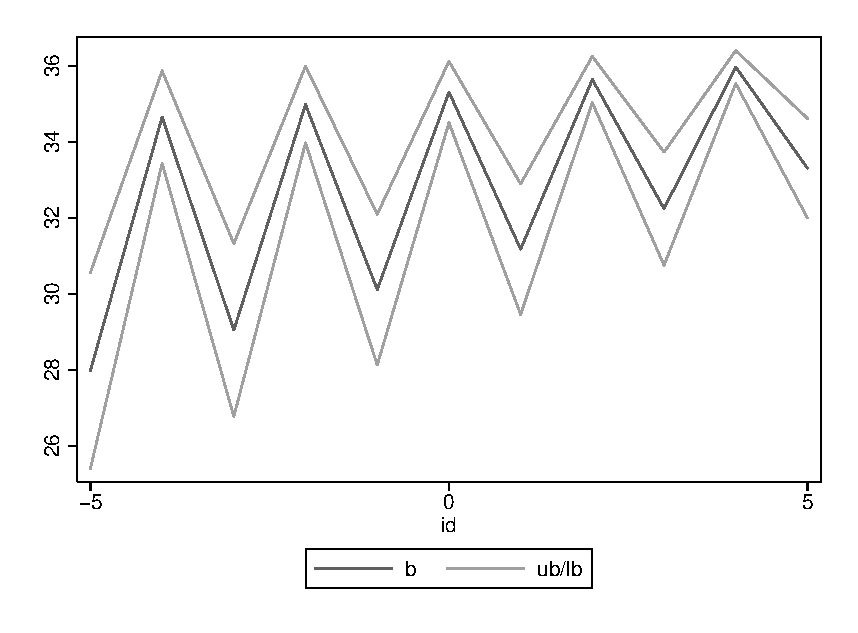
\includegraphics[width=0.8\textwidth]{../figures/volatilityinteraction.eps}
	\centering
	\caption{Marginal effect of $\Delta$house prices on incumbent support across levels of price volatility with 95 pct. Confidence Intervals. Rug plot signifies distribution of observations across the volatility variable.}
\end{figure}


\begin{table}[htbp]\centering
\def\sym#1{\ifmmode^{#1}\else\(^{#1}\)\fi}
\caption{Estimated effects of house prices on electoral support for governing parties across volatility.}
\begin{tabular}{l*{4}{c}}
\hline\hline
                    &\multicolumn{1}{c}{(1)}        &\multicolumn{1}{c}{(2)}        &\multicolumn{1}{c}{(3)}        &\multicolumn{1}{c}{(4)}        \\
\hline
$\Delta$ house price (positive)&        0.15\sym{**}&        0.10\sym{**}&        0.02        &        0.03        \\
                    &      (0.03)        &      (0.04)        &      (0.03)        &      (0.02)        \\
[1em]
$\Delta$ house price (negative)&       -0.06        &       -0.18\sym{**}&        0.03        &        0.02        \\
                    &      (0.07)        &      (0.07)        &      (0.06)        &      (0.05)        \\
[1em]
Volatility          &       -7.41\sym{*} &       -0.17        &        7.31\sym{**}&       -1.18        \\
                    &      (3.76)        &      (3.31)        &      (2.71)        &      (2.03)        \\
[1em]
$\Delta$ house price (positive) $\times$ Volatility&       -0.09        &        0.08        &        0.05        &        0.04        \\
                    &      (0.12)        &      (0.13)        &      (0.10)        &      (0.07)        \\
[1em]
$\Delta$ house price (negative) $\times$ Volatility&        0.01        &        0.29        &       -0.53\sym{*} &       -0.48\sym{**}\\
                    &      (0.30)        &      (0.26)        &      (0.22)        &      (0.17)        \\
[1em]
\hline Polling Station FE&                    &$\checkmark$        &$\checkmark$        &$\checkmark$        \\
[1em]
Year FE             &                    &                    &$\checkmark$        &$\checkmark$        \\
[1em]
Year FE * Structural factors&                    &                    &                    &$\checkmark$        \\
\hline
Observations        &        4185        &        4185        &        4185        &        4164        \\
RMSE                &        8.47        &        7.17        &        5.71        &        4.76        \\
\hline\hline
\multicolumn{5}{l}{\footnotesize Standard errors in parentheses}\\
\multicolumn{5}{l}{\footnotesize \sym{*} \(p<0.05\), \sym{**} \(p<0.01\)}\\
\end{tabular}
\end{table}





\section{Discussion}

How causally convincing is our results?

Is the negativity bias really a bias? Maybe... maybe not.  ff

Implications for policy makers.

Goodnight!



%Appendikser
%Overvej et om forhold mellem volatilitet og prisændringer
%Overvej et på et andet kontekstuelt niveau - e.g. kommuner - jf. MAUP.
%Overvej et om robusthed af interaktionsled - evt. lav kommuneinteraktioner, og se om effekten stadig holder
%Overvej det samme som sidste om positiv-negativ
%Overvej om vi skal lave et datasæt med "stabile valgsteder" 
%Overvej om vi får samme resultater med statsministerpartiet.





\clearpage

\singlespacing

\bibliographystyle{apa}
\bibliography{library}

\end{document}
